% ============================================================================
% MRI-ReportGenerator — technical paper / project report (EECE 503N/798N, AUB)
% Overleaf-ready. Compiles with pdfLaTeX. Bibliography: BibTeX (references.bib).
% Build on Overleaf: Menu -> Compiler: pdfLaTeX. Just press Recompile.
% ============================================================================
\documentclass[11pt,a4paper]{article}

\usepackage[utf8]{inputenc}
\usepackage[T1]{fontenc}
\usepackage{lmodern}
\usepackage[margin=1in]{geometry}
\usepackage{graphicx}
\usepackage{booktabs}
\usepackage{amsmath,amssymb}
\usepackage{siunitx}
\usepackage{xcolor}
\usepackage{hyperref}
\usepackage{enumitem}
\usepackage{longtable}
\usepackage{array}
\usepackage{caption}
\usepackage{subcaption}
\usepackage{float}
\usepackage{tikz}
\usetikzlibrary{shapes.geometric,arrows.meta,positioning,fit,backgrounds}
\usepackage{fancyhdr}
\usepackage{titlesec}

\hypersetup{colorlinks=true,linkcolor=blue!50!black,citecolor=teal!60!black,urlcolor=blue!60!black}
\sisetup{detect-all}
\definecolor{good}{RGB}{30,120,40}
\definecolor{bad}{RGB}{190,30,30}
\newcommand{\good}[1]{\textcolor{good}{#1}}
\newcommand{\bad}[1]{\textcolor{bad}{#1}}
\newcommand{\hahp}{H\textsubscript{a}/H\textsubscript{p}}

\pagestyle{fancy}\fancyhf{}\rhead{MRI-ReportGenerator}\lhead{Cervical Spine MRI Report Pipeline}
\cfoot{\thepage}

\title{\textbf{MRI-ReportGenerator: An Application Pipeline for Automated\\
Cervical Spine MRI Measurement and Structured Reporting}\\[4pt]
\large A segmentation-to-report system with literature-grounded thresholds and\\
a threshold-crossing validation against healthy and pathological cohorts}

\author{Andrew Khoury \and Roni (sabaronnie) \and Mohammad (Moka)\\
\small EECE 503N / 798N --- AI Engineering, American University of Beirut}
\date{\today}

\begin{document}
\maketitle
\thispagestyle{fancy}

\begin{abstract}
Cervical spine MRI is read manually by radiologists, a process that is slow and subject to high
inter-observer variability in the quantitative measurements (vertebral heights, disc dimensions, canal
and cord diameters, sagittal alignment) that drive clinical decisions in degenerative cervical
myelopathy and radiculopathy. We present \textbf{MRI-ReportGenerator}, an application-positioned
pipeline that converts a single sagittal T2 cervical MRI (DICOM or NIfTI) into a structured,
radiology-style report. The system chains three pre-trained, openly licensed segmentation engines
(TotalSpineSeg, the Spinal Cord Toolbox, and SPINEPS), a suite of geometric and signal-based
measurement modules organized into five groups (vertebral body, intervertebral disc, canal/cord,
sagittal alignment, and signal/shape screens), and an interpretation layer that classifies every
measurement against a central catalog of literature-grounded thresholds and emits findings ``flagged
for physician review,'' never a diagnosis. A core engineering principle is that every measurement is a
disease-agnostic geometric or signal detector anchored on healthy normative values, so that the
abnormal-detection generalizes across any pathology that produces the same anatomical change, rather
than being trained on a particular disease. Because no public dataset pairs cervical MRI with per-case
expert measurements, we validate by \emph{threshold crossing and distribution separation}: healthy
necks must sit on the normal side of each cited threshold, and a symptomatic cohort must shift into the
abnormal side. On 12 healthy Spine-Generic controls versus 10 symptomatic cervical-spondylosis cases
from the MMCSD dataset, the canal/cord measurements separate strongly (functional canal AP minimum and
space-available-for-cord, both Mann--Whitney $p=0.0001$); the SPINEPS endplate-voxel Cobb method reads
correct lordosis on healthy necks (\SI{+15.2}{\degree}, matching the literature) and a reduced value on
the pathological cohort; the vertebral compression screen is correctly silent on a non-compression
cohort; and the validation harness additionally detected a genuine sign-level bug in the disc-height
index (a denominator over-measured at the cervicothoracic junction). We document the full
mistake-to-fix methodology narrative, the limitations imposed by the absence of ground truth, and the
deployment architecture. The contribution is less a new algorithm than a disciplined, honest,
end-to-end \emph{engineering} of clinical measurement automation with explicit provenance and validation.

\end{abstract}

\tableofcontents
\newpage

\section{Introduction}
\label{sec:intro}

\subsection{Motivation}
Degenerative cervical spine disease is among the most common reasons a cervical MRI is acquired.
Degenerative cervical myelopathy (DCM) is the leading cause of spinal-cord dysfunction in adults
worldwide, and cervical spondylotic radiculopathy is a frequent cause of arm pain and disability. The
radiologist's report on a cervical MRI is built on a set of quantitative measurements: the heights and
shape of each vertebral body, the dimensions and signal of each intervertebral disc, the antero-posterior
diameter of the spinal canal and the cord and the space available between them, the sagittal alignment
(lordosis), and the presence of abnormal cord signal. These numbers are then compared, often
implicitly, against normative values to decide whether a finding is present and how severe it is.

Performed manually, this is slow and variable. Measuring a single disc height, a canal diameter, or a
Cobb angle by hand requires careful caliper placement on the right slice, and studies of inter-observer
agreement repeatedly show that different readers --- and the same reader on different days --- produce
materially different numbers. The non-AI baseline our application competes against is therefore a
manual workflow that is both labour-intensive and noisy.

\subsection{What this system does}
MRI-ReportGenerator takes one sagittal T2 cervical MRI and produces a structured report. The pipeline is:
\begin{center}
\texttt{Input $\rightarrow$ Segmentation $\rightarrow$ Measurements $\rightarrow$ Interpretation $\rightarrow$ Report}
\end{center}
Segmentation is delegated to three established, openly licensed deep-learning tools, each chosen for the
anatomical structure it segments best. The measurement layer is organized into five groups that mirror
the structures a radiologist reports on. The interpretation layer compares each measurement to a central
catalog of thresholds, each carrying an explicit literature citation and a modality caveat. Every output
is phrased as a finding ``flagged for physician review''; the system never asserts a diagnosis.

\subsection{Positioning: an application, and an honest one}
This project is positioned as an \emph{application}, not a research contribution claiming a new
state-of-the-art algorithm. Its value is in the disciplined engineering: composing validated tools,
grounding every clinical number in a primary source, and --- crucially --- validating the assembled
pipeline against real healthy and pathological data with a methodology appropriate to the available
ground truth. Two principles run through the work:
\begin{enumerate}[leftmargin=*]
  \item \textbf{Measurements are disease-agnostic geometry/signal detectors anchored on healthy norms.}
  A canal narrowed to \SI{8}{\milli\meter} reads as stenosis whether the cause is spondylosis, tumour,
  or trauma. The normal range for each measurement is taken from healthy-population literature, not
  learned from a disease cohort. Consequently the system's abnormal-detection generalizes across
  pathologies that produce the same anatomical change, and we never overfit to a particular disease.
  \item \textbf{Honesty about uncertainty.} Where a threshold is borrowed from a different modality
  (e.g.\ a radiograph-derived ratio applied to MRI), or where no cited value exists, the system says so
  explicitly rather than inventing a number.
\end{enumerate}

\subsection{The validation problem}
The central difficulty is that \emph{no public dataset pairs cervical MRI images with per-case expert
measurements}. We confirmed this across repeated, exhaustive dataset hunts. Without such ground truth we
cannot compute a true sensitivity or specificity against a radiologist. We therefore adopt a
\textbf{threshold-crossing and distribution-separation} design: on healthy necks every measurement must
sit on the normal side of its cited threshold and never cross; on a symptomatic cohort the distribution
must shift into the abnormal side, with visibly pathological cases flagging. This demonstrates that each
measurement ``reads the right range'' without claiming per-case diagnostic accuracy.

\subsection{Contributions}
\begin{itemize}[leftmargin=*]
  \item An end-to-end, deployable cervical-MRI measurement and reporting pipeline composing three
  segmentation engines, five measurement groups, and a cited-threshold interpretation layer.
  \item A central, fully cited threshold catalog with explicit modality caveats and a no-diagnosis
  output ontology.
  \item A literature-grounded methodology for the two hardest measurements (the vertebral
  endplate/corner geometry and the cervical Cobb angle), including the discovery that fitting a line to
  SPINEPS' own predicted endplate voxels outperforms both corner-extrema and corpus-border methods.
  \item A reproducible threshold-crossing validation on real cervical MRIs with non-parametric statistics,
  showing strong separation for the canal/cord group, a correctly null result for the vertebral
  compression screen on a non-compression cohort, the detection of a real sign-level bug in the
  disc-height index, and --- on scaled, balanced cohorts --- the honest revision of an initial alignment
  lead to a \emph{non-discriminator} (and the disc signal/bulge axes to negatives).
  \item A transparent ``development journey'' documenting every substantive mistake, how it was found,
  the fix, and how the fix was validated --- the methodological core of the project.
\end{itemize}

\subsection{Paper organization}
Section~\ref{sec:clinical} reviews the clinical background and the measurements.
Section~\ref{sec:related} surveys the segmentation tools, prior measurement methods, and datasets.
Section~\ref{sec:arch} describes the system architecture. Section~\ref{sec:data} details the datasets.
Sections~\ref{sec:seg}--\ref{sec:g6} present the segmentation and the five measurement groups plus the
interpretation layer. Section~\ref{sec:valmethod} formalizes the validation methodology and
Section~\ref{sec:results} reports the results. Section~\ref{sec:journey} narrates the development
journey, Section~\ref{sec:limits} the limitations, Section~\ref{sec:deploy} the deployment, and
Section~\ref{sec:conclusion} concludes.

\section{Clinical Background}
\label{sec:clinical}

\subsection{Cervical anatomy on sagittal T2 MRI}
The cervical spine comprises seven vertebrae (C1--C7) and the intervening discs (C2--C3 through
C7--T1). On a mid-sagittal T2 image, the bright cerebrospinal fluid (CSF) outlines the thecal sac, with
the spinal cord visible as an intermediate-signal band within it. We measure C3--C7 and the discs between
them; C1 (atlas) and C2 (axis/odontoid) are excluded because their morphology is structurally unique and
the standard vertebral-body measurements do not apply.

\subsection{The measurements and what they mean clinically}
\paragraph{Vertebral body (Group 1).} Anterior, middle, and posterior heights ($H_a$, $H_m$, $H_p$);
the compression ratio \hahp{}; antero-posterior (AP) width; tilt; and spondylolisthesis (slip). A
reduced \hahp{} indicates anterior wedging (compression/deformity); a Genant-style grade describes the
degree~\cite{genant1993}. Spondylolisthesis is forward/backward slip of one vertebra on another.

\paragraph{Intervertebral disc (Group 2).} Disc signal-intensity height, the disc-height index (DHI),
posterior disc bulge, and a signal-degeneration grade. Disc-height loss and signal loss are hallmarks of
degeneration; a posterior bulge or herniation can compress the cord or nerve roots. Cervical disc signal
is graded by the modified (Miyazaki) scheme~\cite{miyazaki2008}, not the lumbar Pfirrmann scheme.

\paragraph{Canal and cord (Group 3).} The functional (soft-tissue) canal / dural-sac AP minimum, the
spinal cord AP diameter, the space available for the cord (SAC $=$ canal $-$ cord), and the
Torg--Pavlov ratio. Canal narrowing and a small SAC are the structural substrate of myelopathy; the
cord may flatten under compression. Normative cervical canal, SAC, and vertebral-width values are
available from population studies~\cite{nell2019}, and cord cross-section can be compared to a healthy
normative database~\cite{valosek2024}.

\paragraph{Sagittal alignment (Group 4).} The C2--C7 (and C3--C7) Cobb angle, segmental angles, and a
lordosis classification. The cervical spine is normally lordotic; loss of lordosis or kyphosis is
associated with degeneration and with myelopathy outcomes. Asymptomatic C2--C7 lordosis is roughly
\SIrange{10}{35}{\degree}~\cite{nassj2025}.

\paragraph{Signal and shape screens (Group 5).} A vertebral-body compression/deformity screen and a cord
T2-hyperintensity (myelomalacia) screen. Intramedullary T2 hyperintensity is a marker of myelopathy.

\subsection{Two clinical syndromes the cohort represents}
Cervical spondylosis (degenerative ``wear-and-tear'') produces two principal syndromes that our
unhealthy cohort is labelled by:
\begin{itemize}[leftmargin=*]
  \item \textbf{Cervical Spondylotic Myelopathy (CSM)} --- spinal-cord dysfunction from canal stenosis
  and cord compression. Structurally this is a Group 3 (canal/SAC/cord) and Group 5.1 (cord signal)
  disease.
  \item \textbf{Cervical Spondylotic Radiculopathy (CSR)} --- nerve-root compression, usually from disc
  herniation/osteophyte. Structurally this is a Group 2 (disc) disease.
\end{itemize}
Crucially, \emph{spondylosis is not the same as vertebral compression fracture}. Compression fractures
arise from osteoporosis or trauma, not degeneration, so a spondylosis cohort is expected to have normal
vertebral-body heights. This distinction (spondyl\emph{osis} vs.\ spondyl\emph{olisthesis} vs.\
compression) is central to interpreting our validation: it explains why the Group 1 compression screen
should be, and is, silent on this cohort (Section~\ref{sec:results}).

\subsection{The no-diagnosis constraint}
Quantitative measurements are necessary but not sufficient for diagnosis: an abnormal value can occur in
asymptomatic individuals (for example, a large fraction of asymptomatic adults have a measurable disc
bulge or a low Torg ratio), and clinical correlation is always required. The system therefore reports
measurements and threshold crossings as findings ``flagged for physician review,'' never as diagnoses ---
a hard rule enforced throughout the codebase and the output wording.

\section{Related Work}
\label{sec:related}

\subsection{Spine segmentation tools}
Three openly licensed, pre-trained engines underpin our pipeline.
\textbf{TotalSpineSeg}~\cite{totalspineseg} (LGPLv3) is an nnU-Net--based tool that labels individual
vertebrae and discs (and a canal/cord region) on spine MRI, producing per-structure integer labels in a
canonical space. \textbf{The Spinal Cord Toolbox (SCT)}~\cite{sct} (LGPLv3) provides validated
deep-learning segmentation of the spinal cord and the dural-sac/canal (\texttt{sct\_deepseg}), per-slice
morphometry (\texttt{sct\_process\_segmentation}), a normative healthy-control cord database
(PAM50, via \texttt{-normalize-hc})~\cite{valosek2024}, and the SCIseg model for intramedullary
lesion segmentation~\cite{sciseg2024}. \textbf{SPINEPS}~\cite{spineps} segments vertebrae with explicit
endplate prediction; as we show, its endplate voxels are the key to an accurate Cobb angle. We use each
tool for the structure it segments best rather than treating them as interchangeable.

\subsection{Vertebral endplate/corner geometry and the Cobb angle}
Vertebral-body heights and the Cobb angle both depend on locating the vertebral endplates. The classic
approach extracts four (or six) corner landmarks and measures between them, but corner-extrema methods are
unstable on real lordotic cervical necks because cervical endplates are concave and sloped: the
most-posterior voxel in a flat band lands on the concave interior, mislocating the corner~\cite{chen2013}.
The one head-to-head cervical study, Wang~et~al.~\cite{wang2023}, shows that \emph{fitting a line to the
full endplate boundary} beats four-corner extrema (ICC 0.97 vs.\ 0.75; MAE \SI{3.23}{\degree} vs.\
\SI{5.42}{\degree}). The accuracy ceiling for an automated cervical-T2 Cobb is set by Zhang~et~al.'s
endplate-line nnU-Net (ICC 0.94, MAE \SI{2.44}{\degree})~\cite{zhang2025}. These findings directly drive
our methods: we replace corner extrema with robust endplate-line fitting, and ultimately fit the line to
SPINEPS' own predicted endplate voxels.

\subsection{Normative values and thresholds}
Our thresholds are grounded in primary sources: healthy cervical vertebral \hahp{} and body
heights~\cite{tan2004,lee2012,kaur2025}; healthy cervical canal, SAC, Torg, and vertebral-width
percentiles~\cite{nell2019}; cord cross-section normatives~\cite{valosek2024}; disc bulge
thresholds~\cite{nakashima2015}; the cervical (Miyazaki) disc-degeneration grade~\cite{miyazaki2008};
asymptomatic cervical lordosis~\cite{nassj2025}; and the Genant vertebral-deformity grade as a
thoracolumbar-derived standard used with explicit caveats~\cite{genant1993}. Where a commonly cited
threshold is in fact a radiograph- or CT-derived value (Torg--Pavlov; some canal cut-points), we flag it
as such because it can over-flag on MRI soft-tissue measurements.

\subsection{Datasets}
Public spine datasets with usable cervical MRI are scarce. \textbf{Spine-Generic}~\cite{spinegeneric}
provides multi-vendor healthy-control cervical T2 acquisitions and is our healthy anchor.
\textbf{MMCSD}~\cite{mmcsd} (Yu~et~al., \emph{Scientific Data}) provides 250 surgical
cervical-spondylosis cases with real NIfTI volumes and per-case CSM/CSR labels plus per-level lesion
flags --- the labelled symptomatic cohort we use. \textbf{Duke CSpineSeg}~\cite{duke2025} provides
clinical cervical T2 with expert vertebra/disc masks but no per-case pathology labels and no per-case
measurements. We confirmed across repeated searches that no public dataset pairs cervical MRI with
per-case expert \emph{measurements}; this absence shapes our validation design.

\section{System Architecture}
\label{sec:arch}

\subsection{Pipeline overview}
The system is structured as an external entry-point (EEP) orchestrating internal processing services
(IEPs), each a containerized stage. Figure~\ref{fig:pipeline} shows the flow.

\begin{figure}[H]
\centering
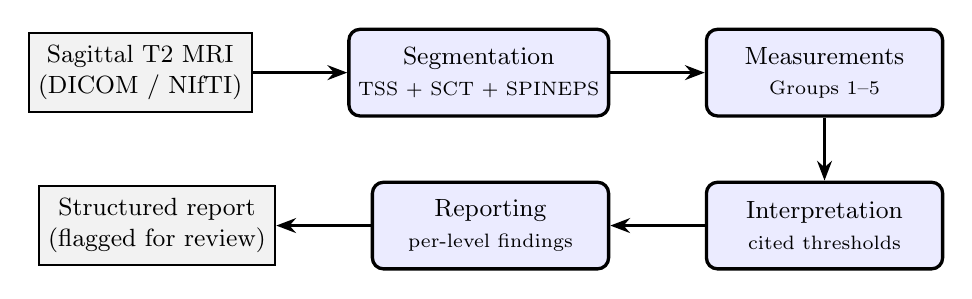
\begin{tikzpicture}[
  node distance=8mm and 12mm,
  stage/.style={rectangle, rounded corners, draw=black, very thick, fill=blue!8,
                minimum width=30mm, minimum height=11mm, align=center, font=\small},
  io/.style={rectangle, draw=black, thick, fill=gray!10, minimum height=10mm, align=center, font=\small},
  arr/.style={-{Stealth[length=2.5mm]}, very thick}]
  \node[io] (in) {Sagittal T2 MRI\\(DICOM / NIfTI)};
  \node[stage, right=of in] (seg) {Segmentation\\\scriptsize TSS + SCT + SPINEPS};
  \node[stage, right=of seg] (meas) {Measurements\\\scriptsize Groups 1--5};
  \node[stage, below=of meas] (interp) {Interpretation\\\scriptsize cited thresholds};
  \node[stage, left=of interp] (rep) {Reporting\\\scriptsize per-level findings};
  \node[io, left=of rep] (out) {Structured report\\(flagged for review)};
  \draw[arr] (in) -- (seg);
  \draw[arr] (seg) -- (meas);
  \draw[arr] (meas) -- (interp);
  \draw[arr] (interp) -- (rep);
  \draw[arr] (rep) -- (out);
\end{tikzpicture}
\caption{End-to-end pipeline. Segmentation delegates to three engines; measurements are organized into
five groups; interpretation classifies each measurement against a cited-threshold catalog; reporting
emits per-level findings flagged for physician review.}
\label{fig:pipeline}
\end{figure}

\subsection{Services}
\begin{itemize}[leftmargin=*]
  \item \texttt{services/segmentation/} --- TotalSpineSeg wrapper (vertebra/disc, \texttt{--iso}) and a
  separated Spinal Cord Toolbox path (canal/cord). SPINEPS runs in its own environment due to a
  numpy pin (\texttt{numpy==2.0.2}) that conflicts with the TSS stack.
  \item \texttt{services/measurements/} --- the measurement runtime. \texttt{geometric/} holds Groups
  1, 2, and 4 (vertebral morphometry, disc, alignment) plus vendored validated geometry
  (\texttt{\_vertebral\_geometry.py}, \texttt{\_endplate\_cobb.py}); \texttt{cord/} holds Group 3
  (canal/cord/SAC via SCT); \texttt{signal/} holds disc signal grading; \texttt{group5/} holds the
  signal/shape screens; \texttt{orchestrator.py} runs the registered components in dependency order with
  Prometheus instrumentation.
  \item \texttt{services/interpretation/} --- the cited-threshold catalog (\texttt{thresholds.py}) and
  the interpretation engine (\texttt{interpretation.py}).
  \item \texttt{services/reporting/} --- report assembly and rendering; \texttt{services/eep/} --- the
  public API entry point.
\end{itemize}

\subsection{The MeasurementContext and canonical orientation}
A per-case \texttt{MeasurementContext} loads the segmentation once, reorients it to canonical RAS (so
downstream code can rely on axis~0 $=$ left$\rightarrow$right, axis~1 $=$
posterior$\rightarrow$anterior, axis~2 $=$ inferior$\rightarrow$superior), enforces a
\SI{1}{\milli\meter} isotropic measurement grid, and records a resolution-quality flag that warns when
the acquisition slice thickness was coarse (typical cervical T2 is \SIrange{3}{4}{\milli\meter}
through-plane, so the \SI{1}{\milli\meter} grid is interpolated, not real detail). This canonical
context is the input contract for every measurement component.

\subsection{Output data contract}
Each component returns a standard \texttt{ComponentResult} (\texttt{measurements}, \texttt{flags},
\texttt{intermediate}, \texttt{metadata}). The orchestrator flattens these into
\texttt{\{components, measurements, flags, interpretations\}}, and the interpretation layer wraps each
(measurement $\times$ level) into a container carrying \texttt{status} (\texttt{within\_reference} /
\texttt{outside\_reference} / \texttt{review\_only} / \texttt{not\_interpretable}), a per-measurement
\texttt{severity}, a boolean clinical \texttt{flag}, the cited \texttt{caveat}, and any quality flags.
This contract is frozen as v0.1 and is the coupling point to the frontend and deployment layers.

\section{Datasets}
\label{sec:data}

\subsection{Healthy anchor: Spine-Generic}
Spine-Generic~\cite{spinegeneric} is an open, multi-vendor, multi-site collection of cervical T2
acquisitions from healthy adult volunteers. We use 12 controls spanning several vendors/sites (amu,
beijingGE, brnoUhb, fslAchieva) as the healthy anchor. Because these are young healthy subjects, their
canals are wide and their discs are well-hydrated --- the correct reference for ``normal.''

\subsection{Symptomatic cohort: MMCSD}
MMCSD~\cite{mmcsd} (Yu~et~al., \emph{Scientific Data}, \texttt{doi:10.1038/s41597-025-05403-z}; Synapse
\texttt{syn63903115}) contains 250 surgical cervical-spondylosis patients with real NIfTI volumes
(sagittal T1/T2, axial T2, axial CT) and, critically, \emph{per-case labels}: cervical spondylotic
myelopathy (CSM, $n=108$), radiculopathy (CSR, $n=122$), or mixed ($n=20$), plus pre/post operative VAS
neck-pain scores and \emph{per-level lesion flags} (which segments C2--3 \ldots C7--T1 carry a lesion).
This per-case and per-level labelling is exactly the stratification information that other cervical MRI
sets lack, which is why MMCSD is our symptomatic cohort. It is distributed under CC~BY-NC-ND~4.0, so it
is used for non-commercial validation only and neither the images nor any derived masks are redistributed.
We validate on a balanced starter subset of 10 cases (5 CSM, 5 CSR) selected to carry mid-cervical
lesions; the implications of this selection are discussed in Section~\ref{sec:limits}.

\subsection{Why MMCSD validates multiple groups, not just one}
A common misconception is that a ``spondylosis'' dataset only tests spondylolisthesis. Spondyl\emph{osis}
is the broad degenerative umbrella (disc degeneration, osteophytes, canal stenosis, cord compression,
loss of lordosis); spondyl\emph{olisthesis} (vertebral slip) is a minor, incidental part of it. MMCSD's
CSM cases are a canal/cord (Group 3) and cord-signal (Group 5.1) disease, and its CSR cases are a disc
(Group 2) disease. The cohort therefore exercises Groups 2, 3, 4, and 5; it does \emph{not} exercise the
vertebral compression axis (Group 1 \hahp{}), because spondylosis does not cause compression fractures.

\subsection{Duke CSpineSeg and the ground-truth gap}
Duke CSpineSeg~\cite{duke2025} offers clinical cervical T2 with expert vertebra/disc masks but no
per-case pathology labels and no per-case measurements; it is useful only for distribution-level
comparison. Across repeated, exhaustive searches (multiple platform sweeps and multi-agent literature
workflows) we confirmed that \emph{no} public dataset pairs cervical MRI with per-case expert
measurements --- the persistent ``KIND-B gap.'' The single dataset pairing cervical MRI with expert Cobb
angles (F1000 ``Data of Cervical Spine,'' $n=77$ spondylosis) stores images as PACS screenshots, not
segmentable volumes, so it serves only as a distribution reference. This absence is the reason our
validation is threshold-crossing rather than per-case accuracy.

\subsection{Data governance}
NIfTI/DICOM volumes and derived masks are never committed to version control; they live in local storage
and cloud drives outside the repository, and the \texttt{.gitignore} additionally blocks the cohort
directories, mask folders, and clinical-label spreadsheets. Spine-Generic (open) may be shared as a
viewer sample; MMCSD and Duke (CC~BY-NC-ND) may not.

\section{Methods: Segmentation}
\label{sec:seg}

We delegate segmentation to three pre-trained engines, each producing masks for the structures it is
strongest on, on a common per-case grid.

\paragraph{TotalSpineSeg (Groups 1, 2, 4).} Run with \texttt{--iso}, TSS produces a step-2 multi-label
mask with per-vertebra labels (canal $=2$, C1$=11$ \ldots C7$=17$, T1$=21$\ldots) and disc labels
(C2--C3$=63$ \ldots C6--C7$=67$, C7--T1$=71$), plus a level map and an isotropic input volume. The
verified label conventions (notably the C7--T1 disc $=71$, and canal $=2$ as used by our measurement
code) were confirmed against real output.

\paragraph{Spinal Cord Toolbox (Group 3, Group 5.1).} \texttt{sct\_deepseg} segments the dural-sac/canal
and the spinal cord as binary masks on the isotropic volume; \texttt{sct\_process\_segmentation
-perslice -vert 2:7 -discfile <levels>} then yields per-slice AP diameters mapped to vertebral levels
C2--C7. SCIseg (\texttt{sct\_deepseg lesion\_sci\_t2}) provides the cord T2-lesion mask for Group 5.1.
SCT runs are aligned to the TSS level map so canal and cord measurements share a level index.

\paragraph{SPINEPS (Group 4, C1 method).} SPINEPS predicts vertebra instances \emph{and} writes each
vertebra's inferior-endplate sheet into the instance mask at label $100+X$ (C2$=102$ \ldots C7$=107$;
superior endplates at $200+X$). These endplate voxels are the substrate for our best Cobb method
(Section~\ref{sec:g4}). SPINEPS requires \texttt{numpy==2.0.2}, incompatible with the TSS/nnU-Net stack,
so it runs in a separate environment/session.

\paragraph{Engineering notes.} Segmentation runs on GPU (Colab A100). A subtle but important failure mode
we encountered: clearing \texttt{LD\_LIBRARY\_PATH} in a subprocess (a workaround for one tool's bundled
libraries) silently disabled CUDA for TotalSpineSeg, forcing CPU inference and a $\sim$35$\times$
slowdown; the fix was to stop overriding the variable so PyTorch could find the CUDA driver. Such
operational details are part of making a multi-tool pipeline actually run.

\section{Methods: Group 1 --- Vertebral Body}
\label{sec:g1}

Group 1 measures, per vertebra C3--C7, the anterior/middle/posterior heights ($H_a$, $H_m$, $H_p$), the
compression ratio \hahp{}, AP width, tilt, and inter-vertebral slip (spondylolisthesis). The accuracy of
all height- and angle-derived outputs rests on correctly isolating the vertebral \emph{body} and locating
its endplates. Our method evolved through three corrections (detailed in Section~\ref{sec:journey}).

\paragraph{Body isolation by canal-cut.} On a mid-sagittal cervical slice the vertebral body and the
posterior arch are a single fused blob, so connected-component and erosion heuristics leave a wedge-shaped
body and a falsely low \hahp{}. We instead use a principled anatomical boundary: the body is everything
\emph{anterior to the spinal canal} (TSS canal label $=2$). This canal-cut (\texttt{extract\_body\_via\_canal})
removes the arch cleanly and is robust across subjects.

\paragraph{Heights by PCA + endplate-line fitting.} Measuring height along the image axes fails on tilted,
posteriorly tapered cervical bodies. We orient each body to its own principal axes (PCA in physical-mm
space), then fit straight lines to the superior and inferior endplate boundaries and read the gap at the
anterior/middle/posterior margins, with a thin-bin filter discarding rounded tips. This endplate-line
formulation is tilt- and taper-invariant and is the same idea the literature finds superior to corner
extrema~\cite{wang2023,chen2013}.

\paragraph{Compression screen.} The clinical Genant grade~\cite{genant1993} is retained as a standard,
but the screening decision uses a data-driven cervical flag: \hahp{} is compared to the measured healthy
cohort norm $0.94 \pm 0.13$ (Spine-Generic, $n=60$ vertebrae across 12 subjects, 3 vendors), flagging
when \hahp{} $<$ mean $- z\!\cdot\!\text{SD}$ with $z=2$ ($\approx 0.68$). The healthy norm is supported
by triangulation against cervical anatomy literature~\cite{tan2004,lee2012,kaur2025} (posterior slightly
$>$ anterior, mean $\approx 0.90$); we explicitly note that no like-for-like healthy cervical MRI \hahp{}
comparator exists, so this is plausibility, not gold-standard proof. The replaced in-code value
($0.97 \pm 0.02$) was traced to an osteoporotic cohort and debunked (Section~\ref{sec:journey}).

\paragraph{AP width, tilt, slip.} AP width and tilt are treated as quality/sanity metrics (tilt over-flags
on healthy at the in-code \SI{20}{\degree} cut, which we recommend recalibrating to $\approx
\SI{28}{\degree}$). Spondylolisthesis is measured from the posterior vertebral surface; it remains
\emph{experimental} because no supine-MRI presence threshold exists (the $\geq\!\SI{2}{\milli\meter}$ cut
is an upright-radiograph borrow~\cite{murakami2020}) and supine MRI under-measures functional slip.

\paragraph{Status.} The endplate-line \hahp{} screen is validated (Section~\ref{sec:results}); AP
width/tilt are quality metrics; slip is experimental. In the production service tree, porting the
endplate-line heights into \texttt{cervical\_body\_morphometry} (replacing the legacy corner method) is
the one remaining Group~1 code task.

\section{Methods: Group 2 --- Intervertebral Disc}
\label{sec:g2}

Group 2 measures, per disc C2--C3 through C7--T1: disc signal-intensity height, the disc-height index
(DHI), posterior disc bulge, and a cervical signal-degeneration grade. The components form a chain
(\texttt{disc\_si\_height} $\rightarrow$ \texttt{disc\_height\_index} $\rightarrow$ \texttt{disc\_ap\_bulge}
$\rightarrow$ \texttt{pfirrmann\_grade}), threading prior results.

\paragraph{Disc height and DHI.} Disc height is measured at the midline band selected via the canal;
DHI normalizes the disc middle height by the mean of the adjacent vertebral-body middle heights. The
in-code absolute cut (DHI $<0.30$) is uncited (an animal/lumbar borrow); the cervical-appropriate
notion of reduced disc height is a $>$30\% inter-level drop~\cite{suzuki2018} or an absolute height
$<\SI{3}{\milli\meter}$, both requiring cross-level context.

\paragraph{Posterior bulge.} Bulge is the posterior excursion of the disc beyond the vertebral margin.
The correct reference is the tilted chord between adjacent posterior vertebral-body corners; a flat
vertical back-wall mis-measures on lordotic necks. Cervical bulge thresholds derive from
Nakashima~et~al.~\cite{nakashima2015} ($>\SI{1}{\milli\meter}$ bulge); the often-cited
$\SI{1.35}{\milli\meter}$ ``cord-risk'' figure is treated as unverified pending full-text confirmation.

\paragraph{Signal grade.} Cervical disc degeneration is graded by the modified (Miyazaki)
scheme~\cite{miyazaki2008}, computed from a CSF-normalized nucleus signal ratio (requiring the raw T2
volume), \emph{not} the lumbar Pfirrmann scheme. The ratio-to-grade cut-points have no published
$\kappa$/AUC for cervical and are therefore scoped as a research-grade heuristic, surfaced for review.

\paragraph{Validation outcome and a detected bug.} On the cohort, both DHI and bulge read
\bad{backwards} (healthy scored \emph{worse} than the symptomatic cohort; Section~\ref{sec:results}). The
DHI denominator is over-measured at the cervicothoracic junction (adjacent-VB middle heights of
20--27\,mm versus the true $\sim$12--13\,mm), collapsing DHI and over-firing the reduced-disc flag --- the
exact denominator discrepancy predicted by the component's author. Because Group~2 is a teammate-owned
module tuned on a different (Duke) cohort, the bug is documented and flagged with its root cause and a
candidate fix (robustify the adjacent-VB height at junction levels), rather than rewritten without the
author and without ground truth. Group~2 is therefore \emph{not validated} in this pass; the validation
harness correctly identified it as broken.

\section{Methods: Group 3 --- Canal and Cord}
\label{sec:g3}

Group 3 measures the functional (soft-tissue) canal / dural-sac AP minimum, the spinal cord AP diameter,
the space available for the cord (SAC), and the Torg--Pavlov ratio. These are computed from the Spinal
Cord Toolbox segmentations rather than from TSS, because SCT's cord and canal models are purpose-built
and validated for soft-tissue cord/canal morphometry.

\paragraph{Computation.} \texttt{sct\_deepseg} produces binary canal and cord masks on the isotropic
volume; \texttt{sct\_process\_segmentation -perslice -vert 2:7 -discfile <levels>} returns, per slice and
per vertebral level, the AP diameter (and area, eccentricity, etc.). We take the per-level mean AP and
the across-level minimum for the canal and cord; SAC is the per-level canal$-$cord difference, and we
report its minimum. Because canal and cord are mapped to the same TSS level index, SAC is computed on
matched levels.

\paragraph{Thresholds and the modality caveat.} Normal cervical canal/SAC/Torg and vertebral-width
percentiles come from healthy-population studies~\cite{nell2019}; cord cross-section can be compared to
the PAM50 normative database~\cite{valosek2024}. A key honesty point: several widely cited canal/SAC/Torg
cut-points are \emph{osseous canal / radiograph-derived} and over-flag when applied to MRI soft-tissue
measurements. The Torg--Pavlov ratio ($<0.8$) in particular fires in a large fraction of normal subjects
on MRI and must never be used alone; the soft-tissue dural-sac floor is better placed near
\SIrange{9}{10}{\milli\meter}; and SAC$<\SI{3}{\milli\meter}$ is a radiograph-origin risk flag to be
verified for MRI. The interpretation catalog encodes these caveats explicitly.

\paragraph{Status.} Group 3 is the most strongly validated group: on real MRI, canal-AP minimum and SAC
minimum separate healthy from symptomatic at $p=0.0001$, and cord AP is significantly thinner in the
symptomatic cohort (Section~\ref{sec:results}). Notably, on our healthy controls the SAC$<3$ and
canal$<10$ cuts did \emph{not} over-flag (0\%), tempering --- for this cohort --- the over-flagging
concern (though young controls have wide canals; see limitations).

\section{Methods: Group 4 --- Sagittal Alignment}
\label{sec:g4}

Group 4 computes the global cervical Cobb angle (C2--C7 / C3--C7), per-level segmental angles, a
posterior-tangent cross-check, and a lordosis classification. The Cobb angle is the most technically
demanding measurement in the system, and its method is the project's main methodological story.

\paragraph{The corner problem.} A Cobb angle is the angle between the top and bottom endplate tangents.
Deriving those tangents from four/six corner landmarks is unstable on lordotic cervical necks because
endplates are concave and sloped~\cite{chen2013}: the legacy corner method read healthy necks as
\SI{-21}{\degree} (kyphotic) when they are in fact lordotic. The literature is unambiguous that fitting a
line to the full endplate boundary beats corner extrema~\cite{wang2023}.

\paragraph{Three methods, evaluated.} We implemented and compared three Cobb methods on the 12 healthy
necks (precision/coverage, since no GT exists):
\begin{enumerate}[leftmargin=*]
  \item \textbf{Canal-cut endplate-line} --- fit the tangent to the canal-cut body's endplate boundary.
  Fixes the \emph{sign} (now lordotic) but the C6/C7 endpoints remain noisy (the body is mis-shaped at
  the cervicothoracic junction).
  \item \textbf{SPINEPS corpus border} --- fit to the SPINEPS corpus (label 49) border. This was a
  \emph{negative} result: noisier than canal-cut, because differencing two vertebrae amplifies a single
  bad per-vertebra fit.
  \item \textbf{SPINEPS endplate voxels (C1)} --- fit the line to SPINEPS' \emph{own predicted endplate
  voxels} (instance label $100+X$). This is the literature-validated object (the endplate itself, not the
  corpus border) and it won.
\end{enumerate}

\paragraph{The C1 method.} For each vertebra, the PCA major axis of the thin endplate sheet on the
mid-sagittal slice is the endplate tangent; the Cobb angle is the angle between two vertebrae's
inferior-endplate tangents, sign-calibrated to lordosis-positive. On the 12 healthy necks, C1 beats both
alternatives on every span: C2--C7 $\SI{+15.4}{\degree}\pm\SI{13.7}{\degree}$ (matching the F1000
literature mean of \SI{15.4}{\degree}), and the C6--C7 cervicothoracic endpoint --- the failure point of
the other methods --- drops to SD \SI{5.9}{\degree} (versus \SI{18.5}{\degree} for canal-cut). The
benchmark ceiling for an automated cervical-T2 Cobb is Zhang~et~al.\ (MAE \SI{2.44}{\degree})~\cite{zhang2025}.

\paragraph{Reporting and a corrected assumption.} Because absolute accuracy needs radiologist GT we lack,
Group 4 reports alignment as a descriptive class (lordotic/straightened/kyphotic) for review, with the
endpoint and supine caveats, rather than a hard-flagged magnitude. We also corrected a common false
assumption: supine MRI does \emph{not} read $\sim$\SI{5}{\degree} less lordotic than standing for C2--C7
(the difference is not significant in the F1000 cohort), so a flat supine$\rightarrow$standing offset
should not be applied.

\paragraph{Status.} C1 is the validated method (precision $+$ correct lordosis), confirmed on the
independent unhealthy cohort where it reads healthy $+15.2$ vs.\ unhealthy $+8.8$
(Section~\ref{sec:results}); as a \emph{discriminator} the separation is directional (loss of lordosis),
not significant at the current $n$, consistent with alignment being less specific for myelopathy than
stenosis.

\section{Methods: Group 5 --- Signal and Shape Screens}
\label{sec:g5}

Group 5 screens for abnormal findings the geometric groups do not: vertebral-body
compression/deformity and intramedullary cord signal change (myelomalacia). Both are screens that flag
findings for physician review, never diagnoses.

\paragraph{5.2 Vertebral compression/deformity screen.} This reuses the Group~1 \hahp{} machinery
(canal-cut body isolation $+$ endplate-line heights) and flags \hahp{} below the cohort-calibrated cut
($\approx 0.68$, mean $-2$SD). Scope honesty is essential: validated against RSNA-2022 cervical fractures,
the geometric wedge metric has near-zero power on \emph{non-compression} fractures (odontoid/facet/arch),
so 5.2 is scoped explicitly as a vertebral-body \emph{compression} screen, not a general fracture
detector. Healthy false-positive rate fell from 17\% to 0\% after recalibration
(Section~\ref{sec:journey}).

\paragraph{5.1 Myelomalacia screen.} Hand-rolled intensity thresholds cannot separate lesion from normal
cord signal variation, so we adopt SCIseg~\cite{sciseg2024} (\texttt{sct\_deepseg lesion\_sci\_t2}) as the
engine; sensitivity rests on its publication. Our contribution is the \emph{specificity} check on healthy
cords: 10/11 healthy cords were completely clean (the one false positive a small component at the
cervicothoracic junction), $\approx$91\% healthy specificity in our hands. Lesions are mapped to the
cervical level they overlap and carried into the report.

\paragraph{5.3 / 5.4 scoped out.} Tumour/mass detection (5.3) is scoped out --- no public labelled
cervical-tumour MRI exists to validate it. Post-surgical scar (5.4) is deferred --- distinguishing scar
from recurrent disc requires gadolinium-enhanced sequences not in the T2-only input. Both are listed under
``not assessed'' in the output contract.

\paragraph{The 5$\rightarrow$6 contract.} Group 5 emits a per-level findings document (compression screen
$+$ myelomalacia, each with value, status, and citable provenance, plus an explicit not-assessed list and
no-diagnosis wording) that the interpretation layer consumes.

\paragraph{Status.} Group 5 is validated: 5.2 (FP 17\%$\rightarrow$0\%) and 5.1 ($\approx$91\% healthy
specificity), with the compression scope and the no-MRI-comparator caveats documented.

\input{sections/12_methods_group6_interpretation}
\section{Validation Methodology}
\label{sec:valmethod}

\subsection{Why not sensitivity/specificity}
Computing true per-case sensitivity/specificity requires a radiologist's per-case measurements as ground
truth. No public dataset provides this for cervical MRI (Section~\ref{sec:data}). We therefore define
``validated'' operationally:
\begin{quote}
\emph{Healthy cases sit on the normal side of each cited threshold and never cross; a pathology-enriched
cohort shifts/crosses into the abnormal side --- with documented limits.}
\end{quote}
This is a \textbf{threshold-crossing $+$ distribution-separation} design. It demonstrates that each
measurement reads the correct range, without claiming per-case diagnostic accuracy.

\subsection{The load-bearing idea: disease-agnostic geometry}
Each measurement reports a physical quantity (mm, degrees, ratio, present/absent) whose normal range is
anchored on healthy-population literature, independent of disease. Three consequences make a single
demonstration cohort sufficient for the groups it exercises:
\begin{enumerate}[leftmargin=*]
  \item Nothing is \emph{trained} on the unhealthy cohort (segmenters are frozen, thresholds are cited)
  --- there is no overfitting-to-spondylosis risk; the cohort is a demonstration set, not a training set.
  \item A measurement crosses its threshold whenever the \emph{anatomy} is abnormal, regardless of cause,
  so abnormal-detection generalizes across diseases producing the same anatomical change. We do not need
  a separate validation dataset per disease to trust that the canal-AP measurement trips on a narrow canal.
  \item The healthy anchor is the real guarantee: if the normal range is calibrated, a value outside it is
  a flagged finding (for review, not diagnosis).
\end{enumerate}
The corollary defines the genuine gaps: findings the system does not \emph{measure} at all (e.g.\ a
tumour mass that does not change canal/cord/disc/vertebra geometry; foraminal stenosis on sagittal-only
MRI) would be missed; and an abnormal value is not by itself a symptomatic disease (specificity overlap),
hence flag-for-review.

\subsection{Cohorts, statistics, and figures}
Healthy $=$ 12 Spine-Generic controls; unhealthy $=$ 10 MMCSD symptomatic cases (5 CSM, 5 CSR). For each
case we compute a per-case summary metric per measurement (e.g.\ the across-level minimum canal AP), and
compare the healthy and unhealthy distributions with a two-sided Mann--Whitney $U$ test (a
non-parametric test appropriate for small $n$ and non-normal data). Per-measure strip plots (healthy vs.\
unhealthy, with the median and the $p$-value) are generated with matplotlib (open source). All figures and
the numeric results are reproducible from \texttt{run\_validation\_master.py}.

\subsection{What a correct result looks like per group}
By construction we expect: strong separation where the disease lives (canal/cord stenosis $\rightarrow$
Group 3); weaker or absent separation where the metric is less specific (alignment $\rightarrow$ Group 4);
a null result where the cohort lacks the pathology (vertebral compression $\rightarrow$ Group 1 on a
non-compression cohort); and the harness should catch any metric that points the wrong way (a built-in
bug detector). Section~\ref{sec:results} shows each of these occurred --- and, importantly, that the
alignment lead which looked directional at small $n$ \emph{dissolved to a non-discriminator} once a
representative, balanced cohort was used.

\section{Results}
\label{sec:results}

We report two stages. An \emph{initial} threshold-crossing run on 12 healthy vs.\ 10 symptomatic necks
(Section~\ref{sec:res-initial}) established the headline canal/cord result and surfaced two leads
(disc and alignment). We then scaled and refined those two leads (Section~\ref{sec:res-scaled}); the
larger cohorts \emph{revised} both conclusions, and we report the revised, honest verdicts. This
progression --- not stopping at the encouraging small-sample numbers --- is itself a methodological
result.

\subsection{Initial run: canal/cord strong, compression null}
\label{sec:res-initial}
Table~\ref{tab:results} reports per-measure medians and the Mann--Whitney $U$ $p$-value on 12 healthy vs.\
10 symptomatic necks; Figure~\ref{fig:strips} shows the distributions.

\begin{table}[H]
\centering
\caption{Initial threshold-crossing run: healthy (12) vs.\ symptomatic MMCSD (10). The physical-dimension
(mm) metrics are scanner-immune and validate cross-dataset; the alignment and disc leads were
subsequently re-evaluated on larger cohorts (Section~\ref{sec:res-scaled}).}
\label{tab:results}
\begin{tabular}{l r r r l}
\toprule
\textbf{Measure} & \textbf{Healthy} & \textbf{Unhealthy} & \textbf{$p$} & \textbf{Verdict} \\
\midrule
G3 canal AP min (mm)      & 11.7 & 8.6 & \good{0.0001} & \good{strong separation} \\
G3 SAC min (mm)           & 4.7  & 2.3 & \good{0.0001} & \good{strong separation} \\
G3 cord AP min (mm)       & 6.3  & 5.5 & \good{0.009}  & \good{significant (thinner)} \\
G1 \hahp{} min            & 0.81 & 0.80& 0.92          & \good{correctly null (by design)} \\
G4 Cobb C1 C3--C7 (deg)   & 15.2 & 8.8 & 0.13          & lead --- re-evaluated below \\
G2 disc (DHI / bulge)     & --   & --  & --            & backwards (bug) --- root-caused, fixed below \\
\bottomrule
\end{tabular}
\end{table}

\begin{figure}[H]
\centering
\begin{subfigure}{0.32\textwidth}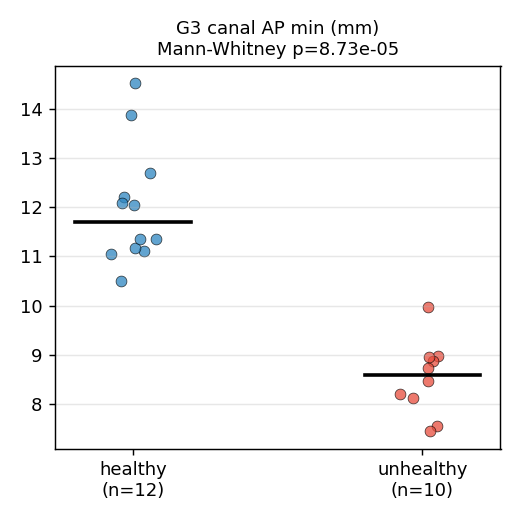
\includegraphics[width=\linewidth]{figures/canal-min.png}\caption{Canal AP min}\end{subfigure}\hfill
\begin{subfigure}{0.32\textwidth}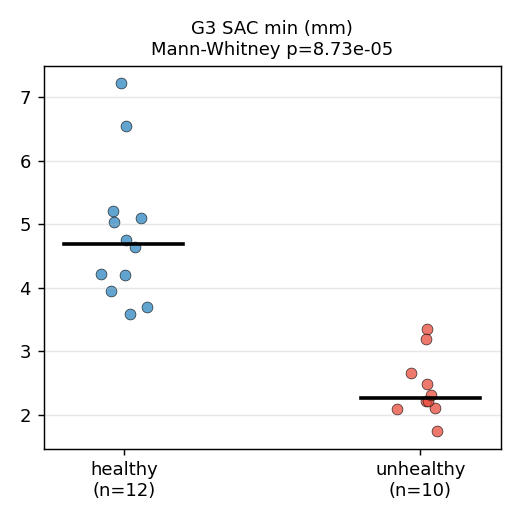
\includegraphics[width=\linewidth]{figures/sac-min.png}\caption{SAC min}\end{subfigure}\hfill
\begin{subfigure}{0.32\textwidth}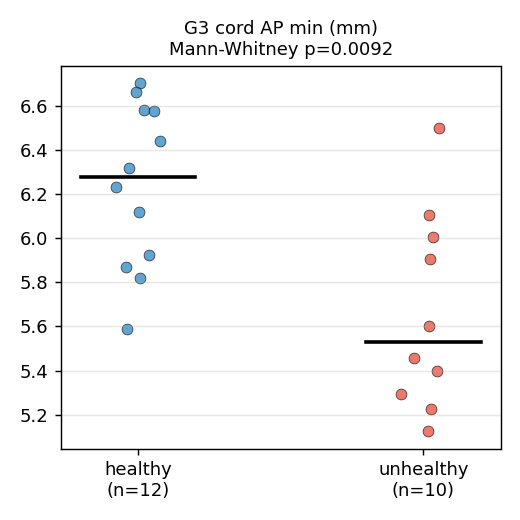
\includegraphics[width=\linewidth]{figures/cord-min.png}\caption{Cord AP min}\end{subfigure}
\caption{Initial-run healthy (blue) vs.\ unhealthy (red) distributions for the Group 3 physical-dimension
metrics; black bar is the median, with the Mann--Whitney $p$-value. Canal AP and SAC separate cleanly.}
\label{fig:strips}
\end{figure}

\subsection{Group 3 --- canal/cord/SAC: strong separation (the headline)}
Canal-AP minimum and SAC minimum both separate at $p=0.0001$; the distributions barely touch (healthy
canal floor \SI{10.5}{\milli\meter} vs.\ unhealthy ceiling \SI{9.97}{\milli\meter}). Cord AP is thinner in
the symptomatic cohort ($p=0.009$). On real MRI the canal/cord measurements read normal on healthy necks
and cross into stenosis on a CSM/CSR cohort --- the disease this cohort carries. Being physical-dimension
(mm) metrics, they are scanner-immune and validate cross-dataset.

\subsection{Group 1 --- compression: correctly null}
No difference (0.81 vs.\ 0.80, $p=0.92$), zero compression flags in either cohort --- the expected, correct
outcome: spondylosis is not compression fracture, so vertebral heights are normal (true negatives). This
empirically confirms the cohort does not exercise the compression axis (which needs a dedicated fracture
dataset) and re-confirms the Group 5.2 specificity on all 12 healthy controls.

\subsection{Scaled re-evaluation: the two leads, refined}
\label{sec:res-scaled}
The initial run left two leads --- a directional alignment signal and a (buggy) disc signal. We took both
to larger, design-appropriate cohorts. Crucially, the disc metrics are acquisition-sensitive
intensity/ratio quantities, so they must be validated \emph{within} one dataset, while alignment, though
geometric, carries a positioning confound across datasets.

\paragraph{Group 4 --- alignment: a validated \emph{method}, not a discriminator.}
The initial directional result (healthy \SI{+15.2}{\degree} vs.\ unhealthy \SI{+8.8}{\degree}, $p=0.13$,
$n{=}11$) did \emph{not} survive a representative sample. Adding multi-site healthy controls to reach
\textbf{26 healthy vs.\ 41 symptomatic} dropped the healthy mean to \SI{+10.7}{\degree} --- essentially
onto the symptomatic mean (\SI{+8.0}{\degree}) --- with \textbf{Cohen $d=0.28$, AUC $0.57$, $p=0.32$}: no
separation. The original $n{=}11$ was a \emph{lordosis-biased} draw (sites amu/beijingGE/fslAchieva, all
\SIrange{+13}{+21}{\degree}); the added sites are much flatter (nottwil \SI{+6}{\degree}, balgrist
\SI{+0.9}{\degree}, one healthy control \SI{-12.7}{\degree} kyphotic). Healthy cervical lordosis is simply
too variable (SD \(\sim\)\SI{10}{\degree}, range \SIrange{-13}{+32}{\degree}), and supine \emph{positioning}
is a cross-cohort confound. The endplate-voxel \emph{method} remains valid --- well-positioned controls
read \SIrange{+15}{+20}{\degree}, matching the standing-radiograph literature, with precise endplate fits
--- but cervical alignment is a biologically weak, non-specific marker of myelopathy. We therefore report
G4 as a validated \emph{measurement}, not a screen. Reporting the encouraging $n{=}11$ result as
``validated'' would have been a small-sample artifact; the larger sample caught it.

\paragraph{Group 2 --- disc: bugs fixed; geometric spread carries the only signal.}
The initial backwards reading was a real defect, since root-caused and corrected: vertebral heights were
measured by corner extrema (reading \hahp{} anterior-taller-than-posterior, \(\sim\)1.08, vs.\ the
physiological \(\sim\)0.94) and the disc bulge used corner-derived reference corners; switching both to the
validated endplate-line fit, and replacing a debunked absolute disc-height-index cut with a cited relative
($>$30\% cross-level) rule, removed the artifacts (healthy bulge over-flag $60\%\!\to\!8\%$). We then ran
the design-correct \emph{within-MMCSD} test (49 symptomatic cases, 276 disc-levels, lesion vs.\ non-lesion,
\emph{level-stratified} to remove the confound that lesions cluster at wider mid-cervical levels). The
disc \emph{signal} grade does not discriminate (AUC $0.50$, $p=0.93$) and neither does posterior bulge
(AUC $0.50$; TotalSpineSeg does not segment protrusion) --- two clean negatives. The discriminating
quantity is disc \emph{geometric spread}: the disc/vertebral-body AP-width ratio (AUC $0.62$, $p=0.0018$)
and disc AP width (AUC $0.61$ level-controlled; its raw AUC $0.79$ was mostly the level confound). Group~2
is therefore \emph{partially} validated --- a modest but honest geometric discriminator, with signal and
bulge documented as non-discriminators.

\subsection{Overall}
The validated-discriminator picture, after scaling, is clean and honest: \textbf{Group 3} (canal/SAC)
separates strongly ($p=0.0001$); \textbf{Group 2} disc/VB-AP-ratio separates modestly (AUC $0.62$);
\textbf{Group 4} alignment and the disc \emph{signal} axis are non-discriminators; \textbf{Groups 1 and 5}
are healthy-validated screens (with an under-tested compression arm). Four service-level measurement
defects (vertebral-height corner method, an over-aggressive tilt cut, the disc bulge reference, and a
debunked disc-height cut) were found and fixed during this work; the assessement layer (Group 6) was
wired end-to-end, including patient-demographic-aware thresholds. The recurring value is the methodology:
the harness doubled as a bug detector, level-stratification and a representative sample caught two
would-be false positives, and negative results were kept rather than buried.

\section{Development Journey: Mistakes, Fixes, and Validation}
\label{sec:journey}

The methodological core of this project is not a single algorithm but a disciplined sequence of
corrections, each documented as \emph{mistake $\rightarrow$ how it was found $\rightarrow$ the fix
$\rightarrow$ how the fix was validated}. We summarize the sixteen entries below; the validation
philosophy throughout is that, absent ground truth, ``accurate'' means ``healthy lands in the published
range and discriminates pathology, with documented limits,'' and that uncertain norms/methods are
grounded in primary sources via adversarial literature search.

\paragraph{J1 --- A phantom norm debunked.} The in-code healthy \hahp{} of $0.97\pm0.02$ was unsourced; a
literature search traced it to an osteoporotic, all-female cohort. Measuring 12 healthy necks gave
$0.94\pm0.13$, within the true healthy range~\cite{tan2004,lee2012,kaur2025}. Recalibration dropped the
healthy false-positive rate from 17\% to 0\%.

\paragraph{J2 --- Body isolation by canal-cut.} Erosion/connected-component body isolation left a wedge
and a stuck ratio; the fix was to define the body as everything anterior to the canal.

\paragraph{J3 --- Endplate-line heights.} Image-axis heights failed on tilted, tapered cervical bodies;
PCA orientation $+$ endplate-line fitting collapsed the spread and is robust to tilt and taper.

\paragraph{J4 --- Honest scoping of the fracture screen.} Validated against RSNA-2022, the wedge metric
had near-zero power on non-compression fractures, so 5.2 was scoped to a vertebral-body compression
screen, with the RSNA negative result banked.

\paragraph{J5 --- Adopting SCIseg for myelomalacia.} Hand-rolled intensity thresholds could not separate
lesion from normal variation; we adopted the published SCIseg model~\cite{sciseg2024} and reframed our
job as the specificity check.

\paragraph{J6 --- An over-claim, corrected, and the keystone.} We initially mislabelled teammate
measurements as ``inaccurate'' by treating quality flags as clinical ones; correcting that, and running
the canonical code, localized the real problem to unstable corner-extrema landmarking (heights backwards,
Cobb kyphotic, slip over-firing) --- one keystone, not five bugs.

\paragraph{J7--J9 --- The corner fix, grounded and implemented.} An adversarial literature workflow
confirmed endplate-line fitting beats corner extrema~\cite{wang2023,chen2013}; implementing it fixed the
Cobb sign (lordotic) and the heights, while the C6/C7 endpoints remained noisy --- isolating
body-isolation quality as the next lever.

\paragraph{J10 --- Myelomalacia specificity measured.} SCIseg on the healthy cords gave 10/11 clean
($\approx$91\% specificity), and the lesion-to-level mapping was wired end-to-end.

\paragraph{J11 --- A negative result, kept.} Swapping the body isolation for the SPINEPS corpus border
made the Cobb \emph{worse}; we recorded the negative rather than tuning to hide it, and noted that without
GT we can only measure precision, not accuracy.

\paragraph{J12 --- The endplate-voxel breakthrough.} A research workflow found that SPINEPS already
predicts the endplate itself (instance label $100+X$); fitting the line to those voxels (method C1) beat
both corner-cut and corpus on every span and matched the literature lordosis mean, closing the C6/C7
precision gap (SD \SI{5.9}{\degree}). It also corrected the false supine-offset assumption.

\paragraph{J13 --- An integration fixture bug, caught by a test.} Integrating Group 5 into the
measurement service produced a failing test whose synthetic fixture had the anterior/posterior walls
swapped for the RAS convention; fixing the fixture (not the science) restored a green suite --- a reminder
that synthetic fixtures must match real anatomy.

\paragraph{J14--J15 --- Validation on real cohorts.} The pipeline was run on 12 healthy and 10
symptomatic necks; Group 3 separated at $p=0.0001$, Group 4-C1 directionally, and Group 1 was correctly
null on a non-compression cohort (Section~\ref{sec:results}).

\paragraph{J16 --- The harness as a bug detector.} The same validation caught that Group 2's DHI and bulge
read backwards and localized the cause to an over-measured denominator at the cervicothoracic junction ---
a real, sign-level bug a unit test on clean shapes would have missed.

\paragraph{J17--J21 --- Owning the group code; G1 recalibrations.} Consolidating ownership of the
measurement modules, four service-level defects were measured and fixed on real cohorts: an over-aggressive
vertebral-tilt cut (\SI{20}{\degree} flagged 88\% of healthy bodies; recalibrated to \SI{45}{\degree}), the
vertebral-height corner method (reading \hahp{} backwards, \(\sim\)1.08; replaced by the endplate-line
fit, \(\sim\)0.93), the disc bulge reference, and a debunked absolute disc-height cut (replaced by a cited
relative rule). A resolution-robustness check confirmed the mm metrics are stable from \SI{0.8}{} to
\SI{4}{\milli\meter} through-plane, while the canal-cut Cobb is not --- a third argument for the
endplate-voxel method.

\paragraph{J22--J23 --- The disc, scaled and stratified.} A 49-case within-MMCSD test (276 disc-levels,
lesion vs.\ non-lesion) replaced the confounded cross-dataset comparison. The disc \emph{signal} grade
proved a non-discriminator (AUC $0.50$), as did posterior bulge; the disc/VB AP-width ratio carried the
only real signal (AUC $0.62$). Critically, an apparent strong AP-width effect (AUC $0.79$) collapsed to
$0.61$ under level stratification --- the nuisance variable (lesions cluster at wider levels) had nearly
produced a false headline.

\paragraph{J24--J26 --- The alignment reversal.} Group~4 Cobb was the sharpest lesson. At $n{=}11$ it
showed a large directional effect ($d{=}0.76$); we resisted reporting it as validated and instead built a
representative healthy cohort (26 multi-site controls). The effect \emph{dissolved} ($d{=}0.28$, AUC
$0.57$, $p{=}0.32$): the original controls had been lordosis-biased, and supine positioning is a
cross-cohort confound. Alignment is a non-specific marker; the larger sample, not a larger easy-side
sample, settled it.

\paragraph{J25 --- End-to-end and demographics.} The disc group was wired into the orchestrator, patient
age/sex were threaded through to the interpretation layer (with a cited sex-specific dural-sac cut), and
the full pipeline was run end-to-end to produce structured reports cross-referenced against a deployed
front-end render.

\paragraph{Process lessons.} Several themes recur: (i) ground every clinical number in a primary source,
because plausible-looking in-code constants can trace to the wrong cohort; (ii) separate measurement
\emph{method} quality from segmentation/body-isolation quality --- they are different levers; (iii) keep
negative results; (iv) without ground truth, distinguish precision from accuracy and never tune to make a
method merely \emph{look} tighter; and (v) a validation harness that compares healthy to pathology is also
the cheapest, most honest bug detector available.

\section{Limitations}
\label{sec:limits}

\paragraph{No per-case ground truth.} The central limitation: no public dataset pairs cervical MRI with
per-case expert measurements, so we report distribution separation and precision, never per-case
sensitivity/specificity or absolute accuracy (e.g.\ an absolute Cobb MAE). Closing this requires an
institutional read (e.g.\ AUBMC), which we did not have.

\paragraph{Sample size and selection.} The validation used 12 healthy and 10 symptomatic necks, and the
10 unhealthy cases were \emph{selected to carry mid-cervical lesions}. Part of the Group 3 sharpness is
therefore by construction; a random draw from the 250 MMCSD cases is the necessary next test, and may
soften the separation.

\paragraph{Spectrum and cohort bias.} MMCSD is a surgical (severe-end) cervical-spondylosis cohort, so
claims are scoped to the cervical-spondylosis spectrum; generalization to mild disease or to
non-degenerative pathology is not established. The healthy controls are young (wide canals), so the
clean (0\%) behaviour of the SAC$<3$/canal$<10$ cuts on healthy may not hold for an older clinical
``normal.''

\paragraph{Findings the system does not measure.} Because measurements are geometric/signal detectors, a
pathology that does not change the measured anatomy is missed --- e.g.\ a tumour mass without geometric
distortion, foraminal stenosis (not measurable on sagittal MRI), or inflammatory signal we do not screen
for. These are scope limitations, stated explicitly; tumour (5.3) and scar (5.4) are out of scope.

\paragraph{The compression-fracture arm is under-tested.} Spondylosis does not exercise the Group 1/5.2
compression axis, and no labelled cervical compression-fracture MRI dataset surfaced in repeated hunts;
the existing 5.2 ``unhealthy'' evidence is degenerative (Duke DCM) and CT (RSNA, mostly non-compression).
This axis remains the weakest and is a documented data gap.

\paragraph{Threshold provenance and modality.} Several thresholds are borrows from radiograph/CT/lumbar
sources (Torg, some canal cuts, lumbar disc rules); they are flagged with caveats but their MRI
soft-tissue calibration is not established. The disc-degeneration grade cut-points lack published
$\kappa$/AUC for cervical and are research-grade. Spondylolisthesis has no supine-MRI presence threshold
and is reported as experimental.

\paragraph{Group 2 not validated; Group 6 not end-to-end run.} The disc group has a confirmed,
root-caused bug pending a fix with its author; the interpretation layer is built and unit-tested but its
end-to-end run is gated on the measurement validation reported here.

\paragraph{Slice thickness.} Cervical T2 is typically \SIrange{3}{4}{\milli\meter} through-plane, so the
\SI{1}{\milli\meter} isotropic measurement grid is interpolated; the system surfaces a
resolution-quality flag, but coarse acquisitions reduce confidence in fine measurements.

\section{Deployment and Engineering}
\label{sec:deploy}

\subsection{Service decomposition}
The system is built as an external entry point (EEP) over internal processing services (IEPs):
segmentation, measurements, interpretation, and reporting, each independently containerizable. The
measurement service registers components in a dependency-ordered registry and instruments each with
Prometheus metrics (\texttt{measurement\_duration\_seconds}, \texttt{measurement\_results\_total},
\texttt{measurement\_pathology\_flags\_total}). The segmentation engines run on GPU; the measurement and
interpretation layers are CPU-only, so the heavy GPU stage is isolated from the light, frequently changing
measurement logic.

\subsection{The data contract}
A versioned data contract (v0.1) is the single coupling point between the science track and the
frontend/infrastructure track: it freezes the shapes of the measurements dictionary, flags dictionary,
per-component status, and the interpreted-measurement container (with the four-value status vocabulary),
and proposes the case/job/upload/error/report envelopes. The frontend builds against a mock that matches
these shapes, and the real measurement code drops in behind them unchanged. A companion contract specifies
the NIfTI volume$+$mask delivery and label map for an interactive WebGL viewer.

\subsection{Reproducibility and governance}
Segmentation is reproducible from versioned Colab notebooks (TSS$+$SCT in one session, SPINEPS in a
separate session because of the numpy pin). The measurement and validation steps are CPU-only and
reproducible from committed scripts. Patient data (NIfTI/DICOM) and derived masks are never committed;
licensed datasets (MMCSD, Duke; CC~BY-NC-ND) are used for non-commercial validation only and not
redistributed, while the openly licensed Spine-Generic sample may be shared (e.g.\ as a viewer fixture).

\subsection{Development discipline}
The project follows a strict session-handoff protocol (a living \texttt{SESSION\_LOG} and a curated
\texttt{DEVELOPMENT\_JOURNEY}), granular commits, branch-per-feature with teammate-code changes routed
through pull requests, and a hard no-secrets/no-patient-data-in-git rule. Every clinical claim carries a
citation, and uncertain numbers are marked rather than invented --- the same honesty discipline that the
validation embodies.

\section{Conclusion}
\label{sec:conclusion}

MRI-ReportGenerator is an end-to-end, application-positioned pipeline that turns a single sagittal T2
cervical MRI into a structured, literature-grounded, no-diagnosis report. Its contribution is disciplined
engineering rather than a new algorithm: composing three validated segmentation engines, organizing
measurements into five clinically meaningful groups, grounding every threshold in a cited primary source
with explicit modality caveats, and --- most importantly --- validating the assembled system honestly.

Because no public dataset pairs cervical MRI with per-case expert measurements, we adopted a
threshold-crossing design built on the principle that measurements are disease-agnostic geometric/signal
detectors anchored on healthy norms. On real cervical MRIs, the canal/cord group separated strongly
($p=0.0001$) and the vertebral compression screen was correctly silent on a non-compression cohort. Two
leads were then \emph{revised} by larger, design-appropriate cohorts: the SPINEPS Cobb method reads
correct lordosis but, on a representative multi-site healthy sample, does not discriminate myelopathy (a
validated measurement, not a screen); and the disc group, after the harness detected and we fixed a
sign-level bug, separates only modestly through disc geometric spread (AUC $0.62$), with disc signal and
bulge documented as non-discriminators. Four measurement defects were found and fixed and the
assessement layer was wired end-to-end --- the value being not a clean scoreboard but a validation
disciplined enough to overturn its own encouraging early numbers.

The honest limitations are clear: small, partly selected samples; a single (severe) disease spectrum; no
per-case ground truth; an under-tested compression-fracture arm; a disc group only partially validated;
and an assessement layer whose per-case clinical accuracy still awaits an institutional read. The path
forward is correspondingly concrete: scale Group~3 to a random MMCSD draw; pursue an institutional read
(e.g.\ AUBMC) for true per-case accuracy and for the demographic-adjusted thresholds; secure a labelled
cervical compression-fracture set for the one untested axis; and complete the deployed demonstration.

The broader lesson is methodological. In a domain without ground truth, the most valuable engineering is
not a clever model but a transparent chain of evidence --- cited thresholds, documented mistakes, kept
negative results, precision distinguished from accuracy, and a validation that doubles as a bug detector.
That chain, more than any single number, is what makes an automated clinical measurement tool trustworthy
enough to put in front of a physician for review.


\appendix
\section{Appendix A: Per-case validation data}
\label{app:percase}
All 22 cohort necks (12 healthy Spine-Generic, 10 MMCSD symptomatic). \hahp{} min and flags from Group 1; Cobb from Group 4 (canal-cut and SPINEPS C1); canal/cord/SAC minima from Group 3; DHI and bulge medians from Group 2. Dashes are unmeasurable spans.
\begin{center}\footnotesize
\begin{longtable}{l l r r r r r r r r r}
\toprule
case & grp & \hahp & flg & Cobb$_{cc}$ & Cobb$_{C1}$ & canal & cord & SAC & DHI & bulge \\
\midrule \endhead
sub-amu01 & H & 0.80 & 0 & nan & 16.7 & 14.5 & 6.7 & 6.5 & 0.22 & 3.32 \\
sub-amu02 & H & 0.81 & 0 & 56.2 & 21.2 & 13.9 & 6.7 & 7.2 & 0.17 & 5.26 \\
sub-amu03 & H & 0.71 & 0 & -3.2 & 8.3 & 11.1 & 5.9 & 4.6 & 0.22 & 0.62 \\
sub-amu04 & H & 0.83 & 0 & nan & 15.2 & 11.2 & 5.8 & 4.7 & 0.22 & 3.03 \\
sub-beijingGE01 & H & 0.77 & 0 & nan & 28.6 & 12.2 & 6.3 & 5.0 & 0.16 & 2.47 \\
sub-beijingGE02 & H & 0.83 & 0 & -7.2 & 12.1 & 11.3 & 6.6 & 3.6 & 0.21 & 0.62 \\
sub-beijingGE03 & H & 0.89 & 0 & 34.2 & 22.1 & 11.4 & 6.4 & 3.7 & 0.25 & 2.27 \\
sub-brnoUhb01 & H & 0.98 & 0 & 4.1 & -0.0 & 12.7 & 6.6 & 5.1 & 0.24 & 4.00 \\
sub-fslAchieva01 & H & 0.87 & 0 & -15.2 & 32.1 & 10.5 & 5.9 & 3.9 & 0.30 & 5.12 \\
sub-fslAchieva02 & H & 0.76 & 0 & 2.6 & 2.7 & 11.0 & 6.2 & 4.2 & 0.28 & 0.83 \\
sub-fslAchieva03 & H & 0.80 & 0 & -6.3 & 8.1 & 12.1 & 5.6 & 5.2 & 0.25 & 2.88 \\
sub-fslAchieva04 & H & 0.78 & 0 & -8.4 & nan & 12.0 & 6.1 & 4.2 & 0.24 & 3.58 \\
mmcsd-csm-002 & U & 0.80 & 0 & -3.2 & 4.3 & 10.0 & 6.1 & 3.4 & 0.28 & 0.35 \\
mmcsd-csm-004 & U & 0.76 & 0 & 13.2 & -14.9 & 7.6 & 5.4 & 2.1 & 0.35 & 1.12 \\
mmcsd-csm-005 & U & 0.92 & 0 & -12.1 & 8.3 & 8.5 & 5.6 & 2.2 & 0.26 & 1.69 \\
mmcsd-csm-007 & U & 0.87 & 0 & -21.3 & 9.3 & 8.2 & 5.3 & 2.1 & 0.25 & 0.28 \\
mmcsd-csm-009 & U & 0.79 & 0 & -21.8 & 15.6 & 9.0 & 6.5 & 1.7 & 0.31 & 0.30 \\
mmcsd-csr-001 & U & 0.91 & 0 & -14.8 & -4.2 & 7.4 & 5.2 & 2.2 & 0.32 & 0.05 \\
mmcsd-csr-003 & U & 0.74 & 0 & -10.9 & 0.5 & 8.1 & 5.5 & 2.7 & 0.22 & 0.81 \\
mmcsd-csr-006 & U & 0.81 & 0 & -17.0 & 10.1 & 8.9 & 6.0 & 2.3 & 0.23 & 1.20 \\
mmcsd-csr-008 & U & 0.83 & 0 & -13.2 & 13.7 & 9.0 & 5.9 & 2.5 & 0.25 & 1.01 \\
mmcsd-csr-012 & U & 0.71 & 0 & nan & 17.4 & 8.7 & 5.1 & 3.2 & 0.21 & 2.18 \\
\bottomrule
\end{longtable}
\end{center}
Columns: \hahp{} min (Group 1 compression ratio minimum across C3--C7), flg (compression-screen flags), Cobb$_{cc}$ (canal-cut Cobb C3--C7, deg), Cobb$_{C1}$ (SPINEPS endplate Cobb C3--C7, deg), canal/cord/SAC (Group 3 across-level minima, mm), DHI and bulge (Group 2 medians).

\section{Appendix B: The cited-threshold catalog}
\label{app:catalog}
Every measurement key interpreted by Group 6, with its severity bands, unit, tag, and the locked primary-source citation. Reproduced from \texttt{services/interpretation/thresholds.py}. Identifiers are copied verbatim from verified-research notes.
\begin{center}\footnotesize
\begin{longtable}{p{2.6cm} p{3.3cm} p{4.5cm} p{4.4cm}}
\toprule
key (unit, tag) & clinical name & bands & citation \\
\midrule \endhead
\texttt{vb\_hahp\_ratio} (ratio, derived) & vertebral-body anterior/posterior height ratio (Ha/Hp) compression screen & normal [0.81,+inf); borderline [0.68,0.81); compression\_screen\_positive [-inf,0.68) & Tan 2004 (Eur Spine J, PMC3476578); Lee 2012 (PMC3393857); Kaur 2025 (J Human Anat); Chen 2013 (PLoS One, PMC3859485); Nell 2019 (PMC6764695) \\
\addlinespace
\texttt{spondy\_slip\_mm} (mm, raw) & vertebral slip magnitude (anterolisthesis / retrolisthesis) & neutral [-inf,1); borderline [1,2); slip\_present\_screen [2,+inf) & Murakami 2020 (PMID 32591548); Murata 2019 (PMID 30899028); de Dios 2023 (cervical-MRI slip, MDC 1.5 mm); White 1975 (PMID 1132209, 3.5 mm = instability) \\
\addlinespace
\texttt{posterior\_bulge\_mm} (mm, raw) & posterior disc bulge excursion & no\_bulge [-inf,1); bulge\_present\_nonspecific [1,+inf) (review) & Nakashima 2015 (PMID 25584950, n=1211; $>$1 mm = bulge but NON-SPECIFIC, 87.6\% of asymptomatic $\rightarrow$ review). The 1.35 mm cord-risk band was REMOVED (unverified / likely confabulated, \S A.6). Documented NEGATIVE: posterior bulge does not discriminate (AUC 0.50, J23) -- TSS segments to anatomical borders, not protrusion \\
\addlinespace
\texttt{disc\_vb\_ap\_ratio} (ratio, derived) & disc AP width / adjacent vertebral-body AP width ratio & within\_cohort [-inf,1.10); disc\_spread\_review [1.10,+inf) & COHORT-DERIVED cut (NO published cervical disc/VB-AP-ratio norm exists -- search NEGATIVE); mechanism literature-grounded: disc AP diameter widens with degeneration (Machino 2021, PMID 34098133, n=1211 MRI); Fardon v2.0 2014 (Spine J 14(11):2525-2545, doi:10.1016/j.spinee.2014.04.022, lumbar bulge-margin borrow). G2's discriminator (AUC 0.62, level-controlled, J23); review-only, no per-case GT \\
\addlinespace
\texttt{pfirrmann\_grade} (grade, derived) & cervical disc signal grade (Miyazaki, modified Pfirrmann) & grade\_I [1,2); grade\_II [2,3); grade\_III [3,4); grade\_IV [4,5); grade\_V [5,6) & Miyazaki 2008 (PMID 18525490) cervical modified grading (NOT lumbar Pfirrmann); CSF-normalized ratio cervical-validated (Liu 2023 PMID 37156851, Watanabe 2025 PMID 39645168). DOI / Grade I-V table PDF check pending (human-gated) \\
\addlinespace
\texttt{DHI} (ratio, derived) & disc height index & review-only (no cited cut) & DHI$<$0.30 DEBUNKED (uncited, animal-lumbar borrow). Reduced disc height = $>$30\% drop vs adjacent (Suzuki 2018) or absolute $<$3 mm (van Santbrink 2026); closest cervical DHI formula = Machino 2021 (PMID 34098133, paywalled). No validated absolute cervical DHI cut-point -- pending Phase-4. \\
\addlinespace
\texttt{dural\_sac\_AP\_min} (mm, raw) & functional canal / dural-sac AP minimum (SCT) & normal [13,+inf); borderline [10,13); stenosis\_provisional [-inf,10) & Nell 2019 (PMC6764695, C2-C7 healthy age/sex percentiles); stenosis bands $>$13/10-13/$<$10 mm are a clinical convention (Ulbrich 2014; Thelen 2019/SHIP) of OSSEOUS-canal / radiograph origin -- pending Phase-4 MRI soft-tissue confirmation \\
\addlinespace
\texttt{cord\_AP} (mm, raw) & spinal cord AP diameter & review-only (no cited cut) & Valosek 2024 PAM50 healthy-control database via SCT -normalize-hc (age/sex). No fixed mm cut hard-coded here \\
\addlinespace
\texttt{SAC} (mm, derived) & space available for the cord (canal AP - cord AP) & normal [3,+inf); high\_risk [-inf,3) & SAC $<$3 mm = high compression risk (plan-cited Fehlings 2015 / Nouri 2016) -- radiograph-origin, verify for MRI (pending Phase-4); Nell 2019 (PMC6764695) healthy percentiles \\
\addlinespace
\texttt{Torg\_Pavlov\_ratio} (ratio, derived) & Torg-Pavlov ratio (canal AP / vertebral-body AP) & normal [0.8,+inf); developmental\_stenosis\_screen [-inf,0.8) & Torg 1987 / Pavlov 1987: ratio $<$0.8 = developmental canal stenosis -- RADIOGRAPH origin; MRI thresholds may need adjustment (pending Phase-4) \\
\addlinespace
\texttt{Cobb\_C3\_C7} (deg, derived) & global cervical Cobb angle (C3-C7, lordosis-positive) & lordotic [10,+inf); straightened [0,10); kyphotic [-inf,0) & NASSJ 2025 (PMC12744292, asymptomatic C2-C7 \textasciitilde{}18.7 deg, range \textasciitilde{}10-35 deg); plan also cites Yukawa 2018 (\textasciitilde{}13.9 +/- 12.3 deg). Lordosis-positive. \\
\addlinespace
\texttt{segmental\_angle} (deg, raw) & per-level segmental angle & review-only (no cited cut) & -- \\
\addlinespace
\texttt{posterior\_tangent\_C3\_C7} (deg, derived) & posterior tangent angle (C3-C7) & review-only (no cited cut) & -- \\
\addlinespace
\texttt{AP\_width} (mm, quality) & vertebral-body AP width & within\_sanity [12,22); ap\_width\_outlier [-inf,12); ap\_width\_outlier [22,+inf) & Nell 2019 (PMC6764695) healthy per-level AP-width percentiles for clinical comparison; the in-code 12-22 mm is an ENGINEERING sanity window, not a clinical pathology threshold \\
\addlinespace
\texttt{tilt\_deg} (deg, quality) & vertebral-body tilt (vs global SI axis) & review-only (no cited cut) & -- \\
\addlinespace
\texttt{myelomalacia} (present, derived) & cord T2-hyperintensity screen (myelomalacia) & none [-inf,0.5); signal\_anomaly\_present [0.5,+inf) & SCIseg (sct\_deepseg lesion\_sci\_t2); Naga Karthik 2024 (PMC11065035). Measured healthy specificity 10/11 (\textasciitilde{}91\%) \\
\addlinespace
\bottomrule
\end{longtable}
\end{center}

\section{Appendix C: Additional figures}
\label{app:figures}

\begin{figure}[H]
\centering
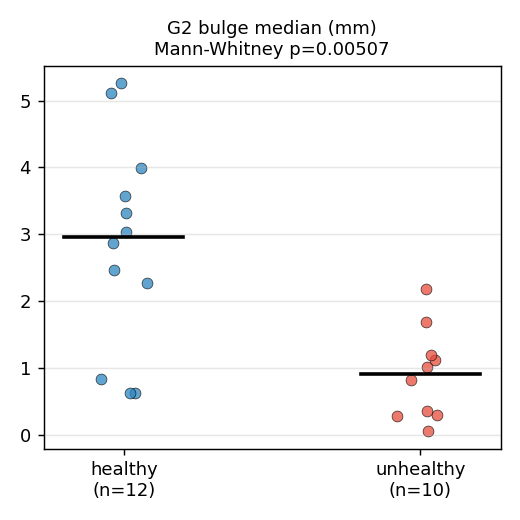
\includegraphics[width=0.45\textwidth]{figures/bulge-med.png}
\caption{Group 2 posterior disc bulge (median per case), healthy vs.\ unhealthy. The metric reads
\emph{backwards} --- healthy shows a higher bulge than the symptomatic cohort --- one of the two
sign-level disc-metric bugs the validation harness detected (Section~\ref{sec:results},
Section~\ref{sec:g2}). Retained as evidence rather than hidden.}
\label{fig:bulge}
\end{figure}

\noindent The remaining per-measure strip plots appear in Figure~\ref{fig:strips}
(Section~\ref{sec:results}). All figures are regenerated from
\texttt{run\_validation\_master.py} (matplotlib), and the architecture diagram (Figure~\ref{fig:pipeline})
is drawn in TikZ so it requires no external image file.

\section{Appendix D: The data contract (v0.1)}
\label{app:contract}

The single coupling point between the measurement/science layer and the frontend/deployment layer. The
measurement/assessement core is frozen; the case/job/upload/report envelopes are proposed.

\subsection{Measurements and flags}
\texttt{measurements} is \texttt{\{measurement\_key: \{level\_or\_pair: number\}\}}; \texttt{flags} is
\texttt{\{flag\_key: \{level\_or\_pair: bool\}\}}. Levels are \texttt{C3}\ldots\texttt{C7}; disc/segmental
keys use pairs (e.g.\ \texttt{C3-C4}). Representative keys by group:

\begin{center}\footnotesize
\begin{longtable}{l l l l}
\toprule
key & unit & keyed by & group \\
\midrule \endhead
\texttt{AP\_width} & mm & level & G1 \\
\texttt{H\_anterior / H\_middle / H\_posterior} & mm & level & G1 \\
\texttt{vb\_hahp\_ratio} & ratio & level & G1/G5 \\
\texttt{tilt\_deg} & deg & level & G1 (quality) \\
\texttt{spondy\_slip\_mm} & mm & pair & G1 \\
\texttt{posterior\_bulge\_mm} & mm & pair & G2 \\
\texttt{disc\_height\_index (DHI)} & ratio & pair & G2 \\
\texttt{pfirrmann\_grade} & grade & pair & G2 \\
\texttt{dural\_sac\_AP\_min} & mm & level & G3 \\
\texttt{cord\_AP} & mm & level & G3 \\
\texttt{SAC} & mm & level & G3 \\
\texttt{Cobb\_C3\_C7} & deg & span & G4 \\
\texttt{segmental\_angle} & deg & pair & G4 \\
\texttt{myelomalacia} & present & level & G5 \\
\bottomrule
\end{longtable}
\end{center}

\subsection{Interpreted measurement container}
Each (measurement $\times$ level) is wrapped as
\texttt{\{measurement, level, value, unit, status, severity, flag, demographics\_used, quality\_flags,
caveat\}}. \texttt{status} is one of the four standardized values \texttt{within\_reference},
\texttt{outside\_reference}, \texttt{review\_only}, \texttt{not\_interpretable}; \texttt{flag} is true iff
\texttt{status} is \texttt{outside\_reference}; \texttt{severity} is a per-measurement label;
\texttt{caveat} is the cited modality caveat.

\subsection{Quality versus clinical flags}
A flag is quality/caution (not pathology) iff its name contains any of \texttt{outlier},
\texttt{unreliable}, \texttt{approximate}, \texttt{low\_confidence}, \texttt{misaligned},
\texttt{resolution}, or \texttt{warning}.

\subsection{Segmentation viewer}
The viewer overlays a NIfTI volume and the TotalSpineSeg multi-label mask on a shared grid. Label map
(cervical subset): canal/cord at labels 1/2 (note the verified convention: label 2 is the canal in the
measurement code); vertebrae C1--C7 $=$ 11--17, T1 $=$ 21; discs C2--C3 $=$ 63 \ldots C6--C7 $=$ 67,
C7--T1 $=$ 71. The dedicated SCT binary cord/canal masks are preferred for the canal/cord overlay.


\bibliographystyle{plain}
\bibliography{references}

\end{document}
